\documentclass[a4paper,12pt]{article}

\usepackage{mathtext}
\usepackage[T2A]{fontenc}
\usepackage[utf8]{inputenc}
\usepackage[russian]{babel}
\usepackage{multirow}
\usepackage{slashbox}
\usepackage{makecell}
\usepackage{graphicx}
\usepackage{physics}
\usepackage{amstext}
\usepackage{caption}
\usepackage{subcaption}
\usepackage{cmap}
\usepackage{float}
%\restylefloat{table}


\title{Лабораторная работа 2}
\author{Калашников Михаил, Б03-205}
\date{}


\begin{document}

\maketitle{Стек и локальные переменные}

\begin{enumerate}

\setcounter{enumi}{0}

\item Сгенерируем листинг для функции, принимающей два аргумента и возвращающей int. Как можно заметить аргументы через регистры esi и edi передаются в стек функции, а возвращаемое значение передается через регистр eax. С флагом -m32 все происходит немного иначе. Аргументы записываются в стек mainа и функция тянется за ними в чужой (mainовский) стек. Возвращаемое значение передается так же.

\begin{figure}[H]
  \centering
  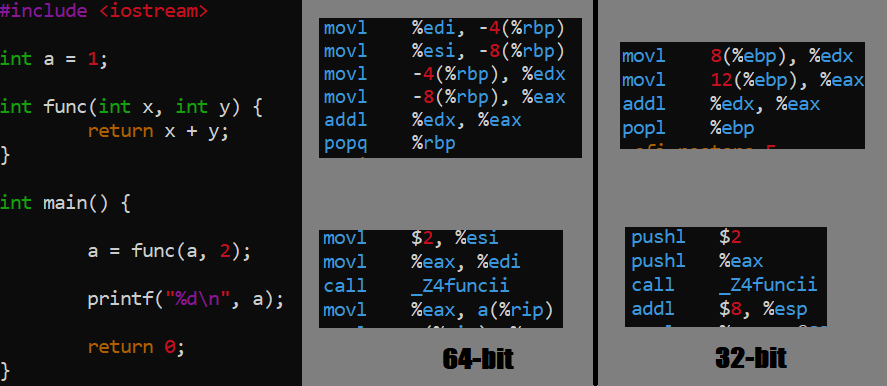
\includegraphics[width=0.8\linewidth]{images/asm2_1.png}
  \caption{К пункту 1}
\end{figure}

\item Локальные переменные и статические массивы работают аналогично. Все значения поочередно добавляются в стек. Перед этим из rsp вычитается нужное количество байтов. При создании динамического массива, в стек сохраняется указатель на него. Обращение к эдементам происходит по адресу, который вычисляется несложным образом.

\begin{figure}[H]
  \centering
  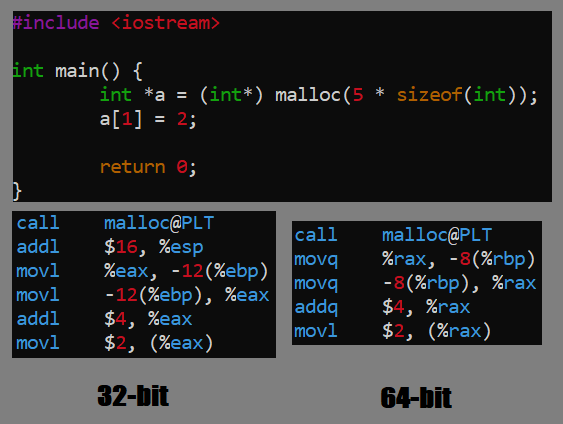
\includegraphics[width=0.8\linewidth]{images/asm2_2.png}
  \caption{К пункту 2}
\end{figure}

\item При создании экземпляра структуры в стек закидываются все ее поля поочередно. Если же создать экземпляр как глобальную переменную, то обращение к полям будет происходить через адрес глобального экземпляра (как на рисунке). Если полем является статический массив, то все работает аналогично. При обращении к нужному элементу массива вычисляется его адрес относительно начала структуры.
Если передать структуру как аргумент, то она запишется в мейновский стек и функция будет обращаться к чужому стеку. При возвращении структуры она вроде как записывается в стек и читается оттуда mainом.
В 32-битной системе все \textbf{гораздо} нагляднее.

\begin{figure}[H]
  \centering
  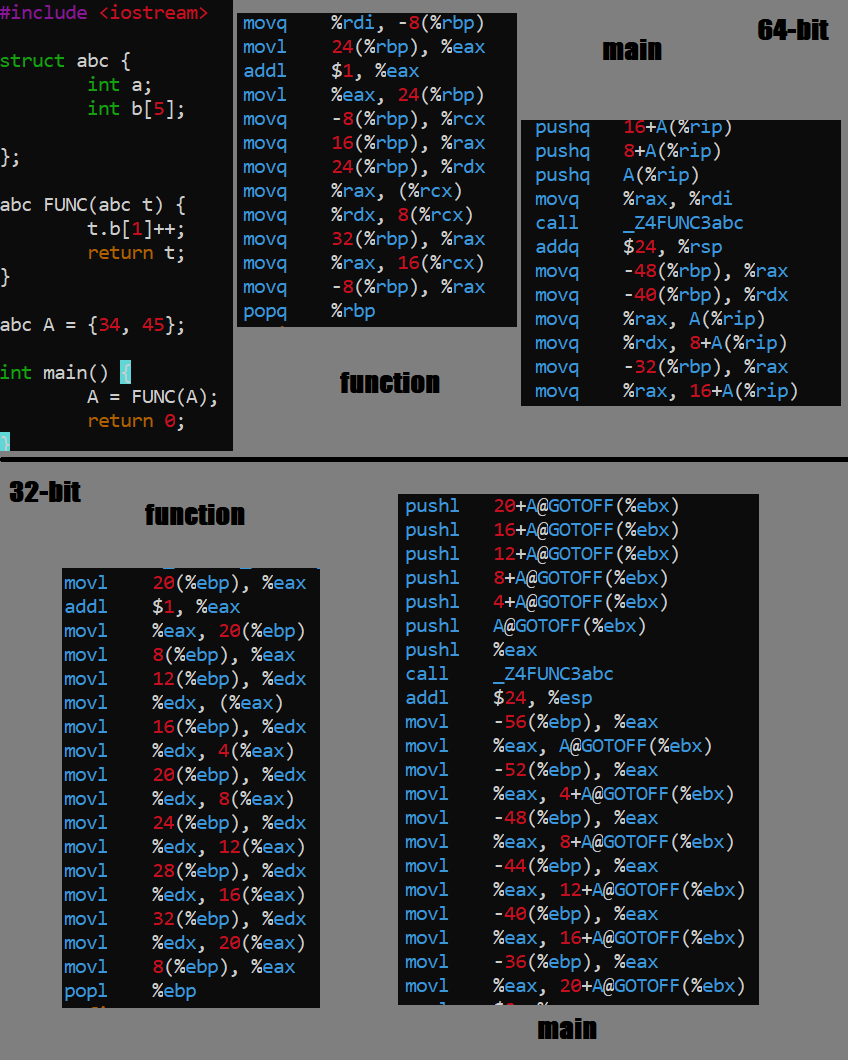
\includegraphics[width=0.8\linewidth]{images/asm2_3.png}
  \caption{К пункту 3}
\end{figure}

\item При передаче структуры по указателю не происходит записывание всей структуры в стек mainа, так как функция сразу знает где структуру искать. В стек записывается только адрес ее начала. Разницу в листинге между передачей по указателю и передачей по ссылке я не нашел. Равны даже размеры файлов с листингами, так что подозреваю что и листинги не полностью идентичны.

\begin{figure}[H]
  \centering
  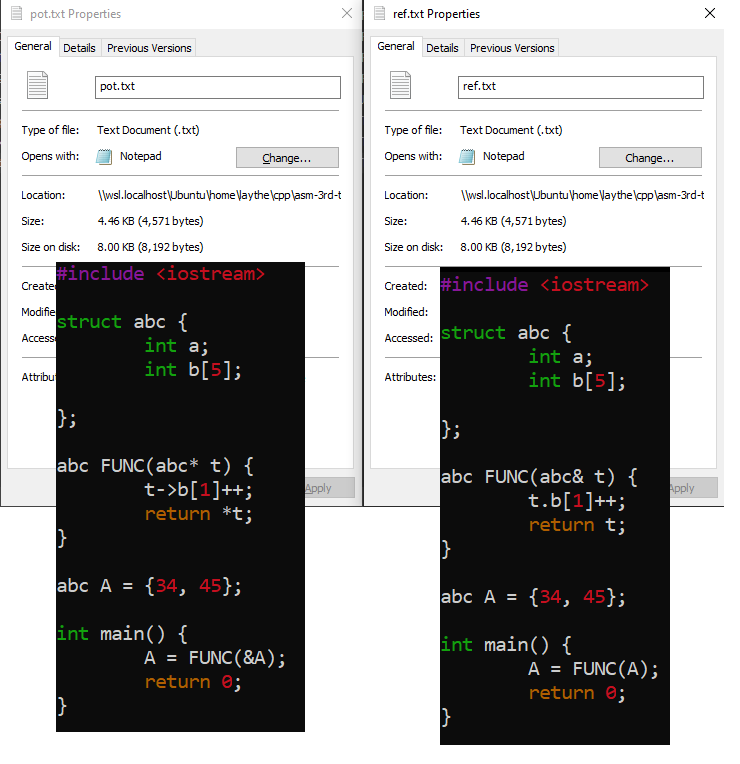
\includegraphics[width=0.8\linewidth]{images/asm2_4.png}
  \caption{К пункту 4}
\end{figure}

\item С жирными структурами работа происходит очень аккуратно. В стек добавляются только необходимые значения. Такой режим работы начинается когда размер структуры превышает 64 байта.

\item Создадим бесконечно-рекурсивную функцию. С помощью ассемблерных вставок реализуем вывод глубины рекурсии в терминал. При такой реализации функция не будет забирать у стека место под работу с printf. То есть на каждом шаге рекурсии будут выполняться два pushq (один от call, второй явный при начале работы функции), а у стека будет съедаться соответственно 16 байт. Зная после какой итерации программа сегфолтунлась, можно найти размер стека:
\[S=523664*16\ байт=8378624\ байт\approx8\ мегабайт\]
Это значение совпадает с ulimit -s, которое тоже равно 8 мегабайтам. :)

\begin{figure}[H]
  \centering
  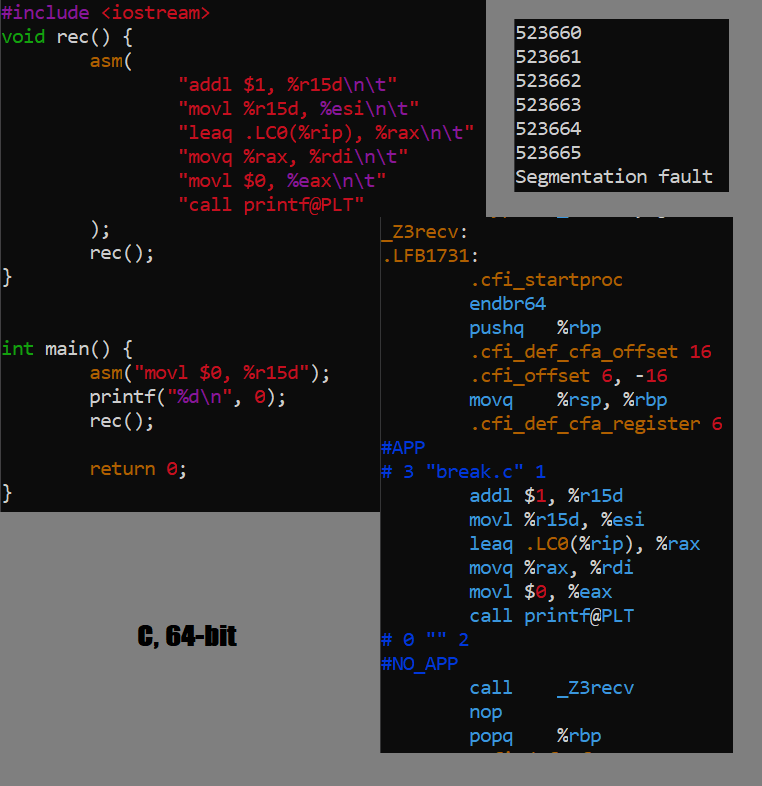
\includegraphics[width=0.8\linewidth]{images/asm2_6.png}
  \caption{К пункту 6}
\end{figure}

\end{enumerate}

\end{document}